\vspace{5mm}
\section{Adaptive $hp$-DG with dynamically-changing meshes}

In this section we present the novel adaptivity algorithm that is the main contribution of the paper.
The algorithm will be applied to compressible Euler equations in Section 3.
We refer to \cite{dubcova,multimesh1,multimesh2} for basic ideas of element-wise assembling in the $hp$-adaptivity settings.
In particular references \cite{dubcova,multimesh2} describe how \emph{multimesh assembling} is 
used to construct adaptive $hp$-FEM/$hp$-DG with dynamically 
changing meshes for transient PDE problems.
In these articles, as well as in this work, we prefer to use Rothe's method to the method of lines for space-time discretization.
The algorithms presented below are implementation-dependent and their concrete 
implementation can be found in the open source library Hermes \cite{hermes}.
\paragraph{Notation}
In the algorithm description, we shall use the following notation. Note that the description presented is for a scalar problem, vector problem differs only in number of components.\\
\\
\begin{tabular}[t]{ll}
$time$&current (physical) time \\
$n$&current time step number \\
$timeStep$&current length of (physical) time step\\
$\mathbf{Space}_n$&DGFE space at time step $n$\\
$\mathbf{SpaceCoarse}_n$&\emph{coarse space}(see below) at time step $n$\\
$\mathbf{Mesh}_n$&mesh (corresponding to $\mathbf{Space}_n$) at time step $n$\\
$\mathbf{Solution}_n$&solution at time step $n$\\
$\mathbf{SolutionCoarse}_n$&$\mathbf{Solution}_n$ projected on $\mathbf{SpaceCoarse}_n$\\
$\mathbf{error}$&calculated relative error estimate\\
$\mathbf{errorTol}$&error estimate tolerance (see below)
\end{tabular}
\paragraph{Algorithm}
This is the algorithm of the solution of nonstationary compressible Euler equations using $hp$-DG. Some terms are marked with a number in square brackets. These terms are explained more thoroughly after the algorithm outline under the appropriate number.
\begin{enumerate}
\item
Initialization:
\begin{itemize}
\item $timeStep$ = a very small initial time step
\item $\mathbf{Space}_1 = \mathbf{Space}_0$ = initial DGFE space - may be very coarse
\item $\mathbf{Solution}_0$ = set according to the initial condition
\item $n$ = 1
\item $time$ = 0.0
\end{itemize}
\item Time-stepping loop:
\begin{enumerate}
\item  Conditionally invoked global mesh derefinement$^{\mathbf{[1]}}$.
\item  Adaptivity loop:
\begin{enumerate}
\item  Assemble$^{\mathbf{[2]}}$ and solve the linear problem on $\mathbf{Space}_n$ obtaining $\mathbf{Solution}_n^{\mathbf{[3]}}$.
\item  (DG specific): detect discontinuities and limit solution $\mathbf{Solution}_n$ to prevent the Gibb's phenomenon.
\item  Project the (limited) $\mathbf{Solution}_n$ to \emph{coarse space} $\mathbf{SpaceCoarse}_n$ $^{\mathbf{[4]}}$ to obtain $\mathbf{SolutionCoarse}_n$.
\item  Calculate error estimate$^{\mathbf{[5]}}$, per element (for adaptivity) and global - $\mathbf{error}$.
\item  is $\mathbf{error}\ <\ \mathbf{errorTol}$ ?
\begin{itemize}
\item (YES)  \begin{enumerate}
\item  As the $\mathbf{Solution}_n$ is captured with the desired tolerance, go to (c).
\end{enumerate}
\item (NO) \begin{enumerate}
\item  Adapt the $\mathbf{Space}_n$.
\begin{itemize}
\item Select elements for refinement$^{\mathbf{[6]}}$
\item For each of the elements selected for refinement, select the optimal $hp$-refinement candidate$^{\mathbf{[7]}}$.
\end{itemize}
\item  Go to (a) - calculate on the adapted space $\mathbf{Space}_n$.
\end{enumerate}
\end{itemize}
\end{enumerate}
\item  Calculate new $timeStep$ value based e.g. on CFL condition.
\item  Set $time = time + timeStep\ \ \ n = n + 1$.
\end{enumerate}
\end{enumerate}

\begin{center}
\line(1,0){450}
\end{center}
$\mathbf{[1]}$ \textbf{Global mesh derefinement} Conditions include e.g. number of DOFs, number of adaptive steps or time steps since last derefinement etc.\\\ \\
The Hermes library offers three options of global derefinement:\\
\begin{itemize}
\item Reset the mesh $\mathbf{Mesh}_n$ to a coarse base mesh $\mathbf{Mesh}_{base}$. Reset the 
      polynomial degrees of all elements to the initial polynomial degree $p_{init}$.
\item Remove $m$ refinement layers uniformly from all elements in the mesh $\mathbf{Mesh}_n$. Here $m$ 
      is usually one, two or at most three. Reset the polynomial degrees of all elements
      to the initial polynomial degree $p_{init}$.
\item Remove just one refinement layer uniformly from all elements in the mesh $\mathbf{Mesh}_n$. 
      Decrease the polynomial degrees of all mesh elements by one.
\end{itemize}
The first option is mathematically the cleanest, meaning that the mesh obtained 
on the new time level are completely independent from the mesh that were
generated during the last time step. The last option is fastest, but the 
sequence of dynamical meshes generated in this way may have on average 
more DOF than needed. The second option is a compromise.\\\ \\
$\mathbf{[2]}$ \textbf{Assembling of the problem} The $hp$-DG assembling requires treating several difficulties:
\begin{itemize}
\item hanging nodes: increases the difficulty of searching element's neighbors for calculating numerical fluxes
\item variable polynomial order: damaged sparsity pattern of the matrix
\item projection-based error estimation: treating overshoots and undershoots very well is a must, otherwise $\mathbf{Solution}_n$ can not be treated as the 'reference' solution.
\end{itemize}
$\mathbf{[3]}$ \textbf{Dynamical meshes} It is noteworthy that one has to use $\mathbf{Solution}_{n-1}$ for the calculation of $\mathbf{Solution}_n$ here.
These solutions, however, are generally defined in different spaces: $\mathbf{space}_{n-1}$, and therefore, projections, or the \emph{multimesh} assembling (see above), must be used.\\\ \\
$\mathbf{[4]}$ \textbf{Projection to \emph{coarse space} $\mathbf{SpaceCoarse}_n$} Here, the \emph{coarse space} is a DGFE space used for error estimate calculation with the following origin: the (reference) space is created from these \emph{coarse space} by uniform mesh refinement and global increase of polynomial order by 1.\\\ \\
$\mathbf{[5]}$ \textbf{Error estimation} Both global and element-wise relative error estimate is calculated using the following:
	$$error_{estimate} = \frac{\mathbf{solution}_{n} - \mathbf{solutionCoarse}_n}{\mathbf{solution}_{n}}$$
$\mathbf{[6]}$  \textbf{$hp$-refinement strategy} As the goal of adaptivity is to find "optimal" $\mathbf{Space}_n$ for capturing ${\mathbf{solution}_{n}}$, we have to apply a strategy what elements to refine based on the calculated element-wise errors. One of the usual strategies is e.g. to refine only top fraction of elements sorted by the largest error. More about these strategies can be found in the literature cited before.\\\ \\
$\mathbf{[7]}$  \textbf{Selecting optimal $hp$-refinement}
Some implementation of the algorithm for determining optimal $hp$-refinements, such as in \cite{derade}, are 
quite complex. Built upon the projection-based interpolation theory,
such approach first finds optimal $hp$-refinement of mesh edges using a 1D
version of the $hp$-adaptive algorithm. The edge refinements then
determine $h$-refinement of elements. Finally, best polynomial
degrees for element interiors are selected. Each step of the algorithm
represents a considerable implementation burden.

We have implemented a much simpler scheme, which is local in the sense
that element refinements are selected without regard to the refinements
of neighboring elements. For all elements $K\in \mathbf{Mesh}_n$ of polynomial
degree $p$ picked by the outer loop we consider the following 
$N = 83$ $hp$-refinement options:
\begin{enumerate}
\item Increase the polynomial degree of $K$ to $p+1$ without spatial subdivision.
\item Increase the polynomial degree of $K$ to $p+2$ without spatial subdivision.
\item Split $K$ into four similar triangles $K_1, K_2, K_3, K_4$.
      Define $p_0$ to be the integer part of $(p+1)/2$.
      For each $K_i$, $1 \le i \le 4$ consider polynomial
      degrees $p_0 \le p_i \le p_0 + 2$.
\end{enumerate}
For each of these $N$ options we perform a standard element-bound $L_2$-projection
of the reference solution $\mathbf{Solution}_{n}$ onto the space of polynomials defined on the element, corresponding to the candidate. The candidate with smallest projection error is selected
for $hp$-refinement of the element $K$.\\

Each of the $N$ projection problems requires the solution of a small
system of linear algebraic equations with a symmetric positive-definite
matrix. The solution of these systems can be further optimized by exploiting
the incremental nature of the Cholesky decomposition algorithm 
and the fact that the spaces in item 3 above are partially embedded. 

\begin{center}
\line(1,0){450}
\end{center}

\paragraph{Example}
We again solve Problem~\ref{ade} but this time, we shall start with a very coarse initial mesh and automatic $hp$-adaptivity will be used. Although the maximum value of the exact solution is $1.0$, due to the presence of undershoots and overshoots, the maximum values here are higher, as was seen already in Section~\ref{sec:DG}. This can be avoided by using a suitable shock capturing method, as it is done in the last chapter with numerical examples for the Euler equations.
\begin{figure}[H]
\begin{center}
\includegraphics[width=0.45\textwidth]{minor_examples/AdaptRelError/Sln1.png}\ \ \ 
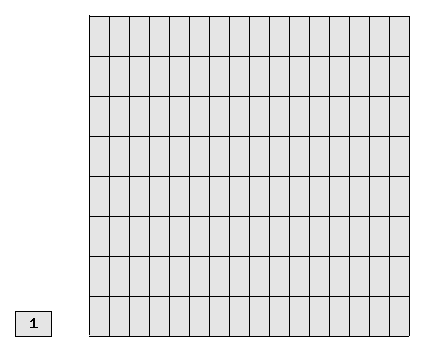
\includegraphics[width=0.44\textwidth]{minor_examples/AdaptRelError/Space1.png}
\end{center}

\caption{Solution $\mathbf{Solution}_1$ calculated on the initial space $\mathbf{Space}_1$ polynomial orders having 512 DOFs, $error_{estimate} = 25.77\%$.}
\end{figure}

\begin{figure}[H]
\begin{center}
\includegraphics[width=0.45\textwidth]{minor_examples/AdaptRelError/Sln2.png}\ \ \ 
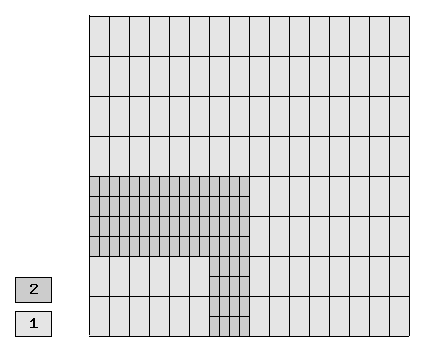
\includegraphics[width=0.44\textwidth]{minor_examples/AdaptRelError/Space2.png}
\end{center}

\caption{Solution $\mathbf{Solution}_3$ and the space $\mathbf{Space}_3$ with polynomial orders having 1152 DOFs, $error_{estimate} = 9.60\%$.}
\end{figure}

\begin{figure}[H]
\begin{center}
\includegraphics[width=0.45\textwidth]{minor_examples/AdaptRelError/Sln3.png}\ \ \ 
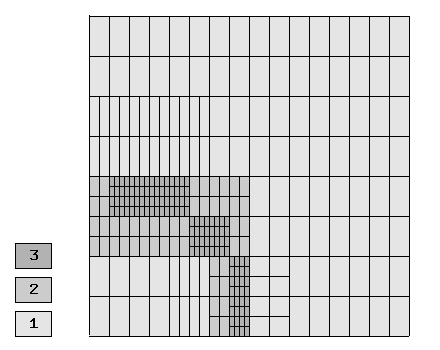
\includegraphics[width=0.44\textwidth]{minor_examples/AdaptRelError/Space3.png}
\end{center}

\caption{Solution $\mathbf{Solution}_5$ and the space $\mathbf{Space}_5$ with polynomial orders having 2992 DOFs, $error_{estimate} = 4.46\%$.}
\end{figure}

\begin{figure}[H]
\begin{center}
\includegraphics[width=0.45\textwidth]{minor_examples/AdaptRelError/Sln4.png}\ \ \ 
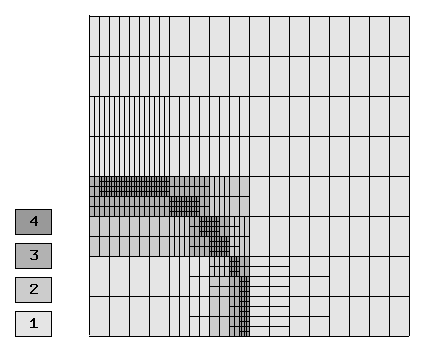
\includegraphics[width=0.44\textwidth]{minor_examples/AdaptRelError/Space4.png}
\end{center}

\caption{Final solution $\mathbf{Solution}_7$ and the space $\mathbf{Space}_7$ with polynomial orders having 9872 DOFs, $error_{estimate} = 2.32\%$.}
\end{figure}
